\subsection{Evaluación de Funciones}
Tomemos como ejemplo la siguiente función:
$$
	F(x) = x e^{-x} \sum_{n=1}^{\infty}\frac{x^n}{n(n!)}	\ \ \ \ \ \ \ \ (x
\ge 0).  
$$

Si queremos conocer las propiedades de $F(x)$ para todo $x$ positivo, la serie
es insatisfactoria en al menos dos puntos de vista.
\begin{enumerate}
	\item Converge lentamente para $x$ grandes.
	\item El número de términos requeridos es del mismo orden que el argumento
dado.
\end{enumerate}

Por ello, uno se encuentra con problemas de escalamiento del problema a medida
que $x$ crece.

Por ello, para resolver el problema, es más directo obtener una ecuación diferencial ordinaria que
satisfaga la función $F(x)$:
$$
F'(x) = \{^{\frac{1-x}{x}F(x) + 1 - e^{-x} \ \ \ \ \ \ (x \neq 0),}_{0 \ \ \ \
\ \ \ \ \ \ \ \ \ \ \ \ \ \ \ \ \ \ (x = 0), }
$$
Con $F(0) = 0$.\\

De ésta forma está claro que este $F(x)$ debe alcanzar 1 para valores largos
de $x$. De hecho, es bastante fácil verlo como una serie diréctamente desde la
ecuación diferencial:
$$
F(x) \thicksim 1 + \frac{1!}{x} + \frac{2!}{x^2} + \cdots
$$

Podemos comprobar que esta última aproximación, se comporta como nuestro F(x) inicial,
mediante un analisis gráfico:

\lstset{basicstyle=\footnotesize, breaklines=true, numbers=left,
frame=shadowbox, rulesepcolor=\color{black}}

F(x) inicial en Matlab:\\
\lstinputlisting{scripts/F1.m}

F(x) aproximado en Matlab:\\
\lstinputlisting{scripts/F2.m}

Código de prueba en Matlab:\\
\lstinputlisting{scripts/test.m}

En donde n:m define el rango a graficar para los valores del argumento x en cada función. N define el limite superior de la sumatoria en la función F(x) inicial
y además define en que termino truncar en la segunda F(x)

Graficando algunos valores para x, podemos darnos cuenta de ésto de manera mas sencilla:

\begin{itemize}

\item $x \in [18,30]$ y N = 50

\begin{center}
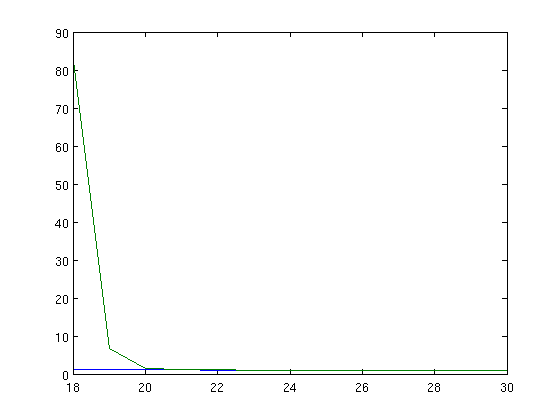
\includegraphics[scale=0.5]{images/2a.png}
\end{center}

\item $x \in [20,30]$ y N = 50


\begin{center}
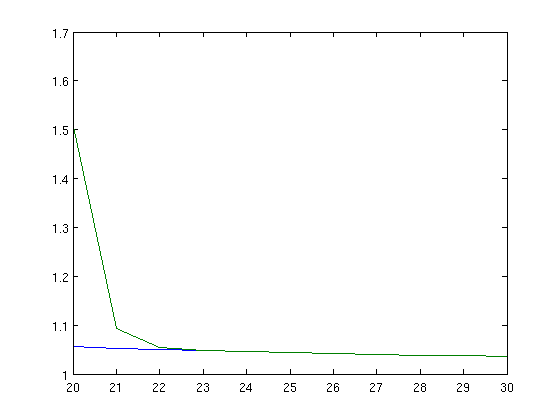
\includegraphics[scale=0.5]{images/2b.png}
\end{center}

\item $x \in [22,30]$ y N = 50


\begin{center}
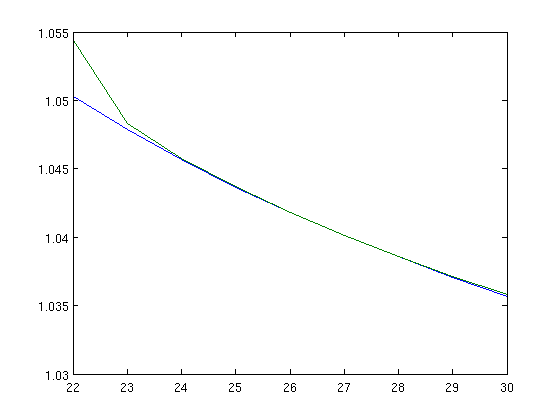
\includegraphics[scale=0.5]{images/2c.png}
\end{center}

\item $x \in [24,30]$ y N = 50

\begin{center}
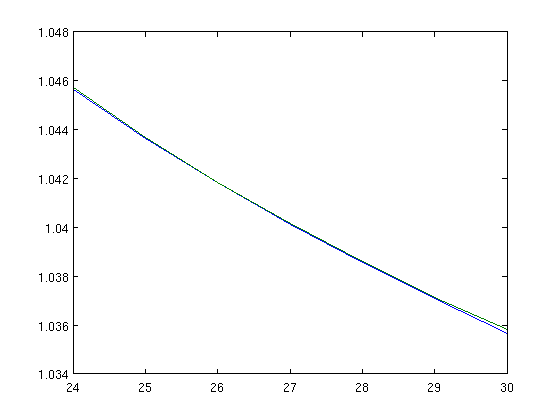
\includegraphics[scale=0.5]{images/2d.png}
\end{center}


Logrando finalmente darnos cuenta que para valores de x grandes:

$$
F(x) = x e^{-x} \sum_{n=1}^{\infty}\frac{x^n}{n(n!)} \thicksim 1 + \frac{1!}{x} + \frac{2!}{x^2} + \cdots
$$


\end{itemize}

La resolución más directa, consistiría en resolver la ecuación diferencial
ordinaria nombrada anteriormente computacionalmente. Esta solución es
fácilmente programable, y resolveria para pequeños y largos valores de $x$
limpiamente. La rutina automaticamente selecciona y ajusta la matriz en $x$
para proveer la presicion especificada y el detalle de la función. Lo único
que se debería analizar más a fondo sería los errores propagados e
inastibilidades de la ecuación diferencial en sí.
